\section{Bot}
\label{sec:module.Bot}


\begin{figure}[bth]
\centering
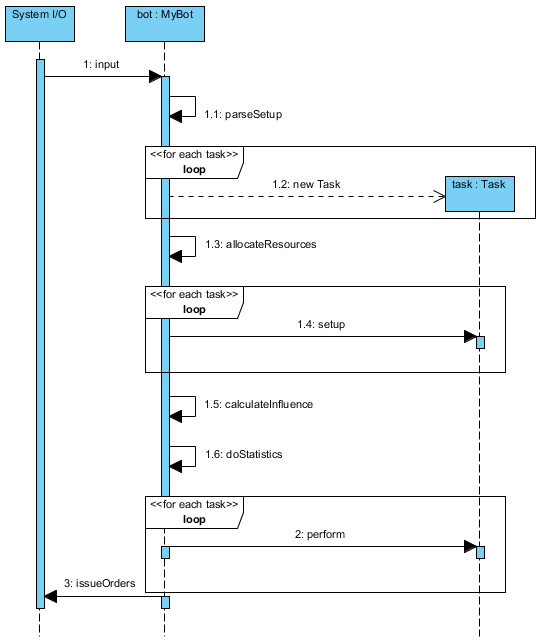
\includegraphics[width=0.9\textwidth]{91_bilder/FirstTurn}
\caption{Ablauf des ersten Zugs des Spiels}
\label{fig:firstTurn}
\end{figure}

\begin{figure}[bth]
\centering
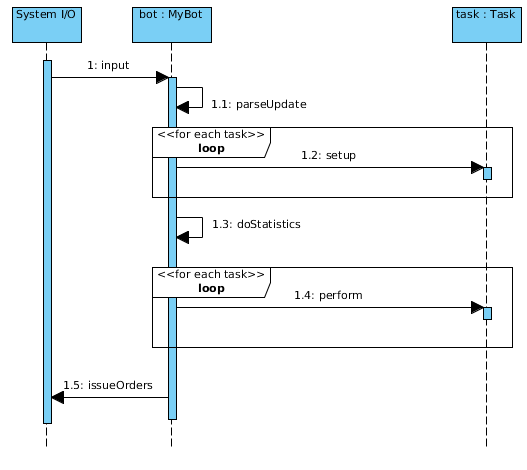
\includegraphics[width=0.9\textwidth]{91_bilder/Turn}
\caption{Ablauf der weiteren Z�ge des Spiels}
\label{fig:turn}
\end{figure}

Als Basis f�r unsere Bot Implementation haben wir den Beispiel-Bot (Klasse Bot.java) verwendet, der im Java-Starter-Package enthalten ist, das von der AI-Challenge-Website heruntergeladen werden kann. Dieser erbt von den Klassen AbstractSystemInputReader und AbstractSystemInputParser, die die Interaktion mit der Spiele-Engine �ber die System-Input/Output Streams kapseln. F�r eine optimierte L�sung k�nnte der Bot auch angepasst werden, indem er selber auf die Streams zugreift. Im Rahmen dieser Arbeit erschien uns das aber noch nicht n�tig.

\subsection{MyBot}
\label{sec:module.Bot.MyBot}




\begin{figure}[bth]
\centering
\includegraphics[width=0.7\textwidth]{91_bilder/Vererbung_bots}
\caption{Vererbung der Bots wobei auf Stufe impl (Implementation) nur MyBot verwendet wird.}
\label{fig:entitiesSearch}
\end{figure}

TODO IMAGE 

\subsection{Ablauf eines Zugs} 
\label{sec:implementation.Bot.Turn}
Abbildung \ref{fig:firstTurn} zeigt den Ablauf des ersten Zugs, w�hrend Abbildung \ref{fig:turn} den Ablauf aller weiteren Z�ge zeigt. 

Jeder Zug beginnt mit dem Einlesen des Inputs vom SystemInputStream. Wenn der Bot das Signal ''READY`` (1. Zug) oder ''GO`` (alle weiteren Z�ge) erh�lt, kann er den gesammelten Input verarbeiten (Methode parseSetup() resp. parseUpdate()). Danach wird die eigentliche Logik des Bots ausgef�hrt.

Im 1. Zug werden dabei Instanzen der Tasks erstellt. Abgesehen davon unterscheidet sich der 1. Zug von diesem Punkt an nicht mehr von allen nachfolgenden Z�gen. Die Tasks werden vorbereitet (Aufruf der jeweiligen setup() Methode; danach werden einige statistische Werte aktualisiert und in jedem 10. Zug auch geloggt. Dann werden die Tasks in der definierten Reihenfolge aufgerufen. Hier wird der L�wenanteil der Zeit verbracht, denn die Tasks enthalten die eigentliche Logik unserer Ameisen.

Zum Schluss werden dann mit issueOrders() die Z�ge der Ameisen �ber den SystemOutputStream an die Spielengine �bergeben.


